\documentclass[tikz,border=12pt]{standalone}
\usepackage[T1]{fontenc}
\usepackage[utf8]{inputenc}
\usepackage{lmodern}
\usetikzlibrary{calc}

\definecolor{ink}{HTML}{243247}
\definecolor{muted}{HTML}{64748B}
\definecolor{fun}{HTML}{7654A3}
\definecolor{str}{HTML}{C17A35}
\definecolor{pro}{HTML}{168A87}
\definecolor{con}{HTML}{3B6FAB}
\definecolor{facefront}{HTML}{DDEFE5}
\definecolor{faceside}{HTML}{C9E4DF}

\definecolor{privacy}{HTML}{566FA5}
\definecolor{privacyfront}{HTML}{E9EDF8}
\definecolor{privacyside}{HTML}{D8E2F3}

\tikzset{
  edge/.style={
    draw=ink, line width=1.15pt, line cap=round
  },
  hidden edge/.style={
    draw=muted!85!black, line width=1.05pt,
    dash pattern=on 3pt off 2.2pt
  },
  vertex/.style={
    circle, draw=white, line width=1.4pt,
    minimum size=8pt, inner sep=0pt
  },
  label box/.style={
    rectangle, rounded corners=3pt,
    draw=#1!70!black, fill=#1!10,
    line width=0.9pt, align=center,
    text width=3.4cm, inner sep=6pt,
    font=\small
  },
  label box/.default=ink
}

\begin{document}
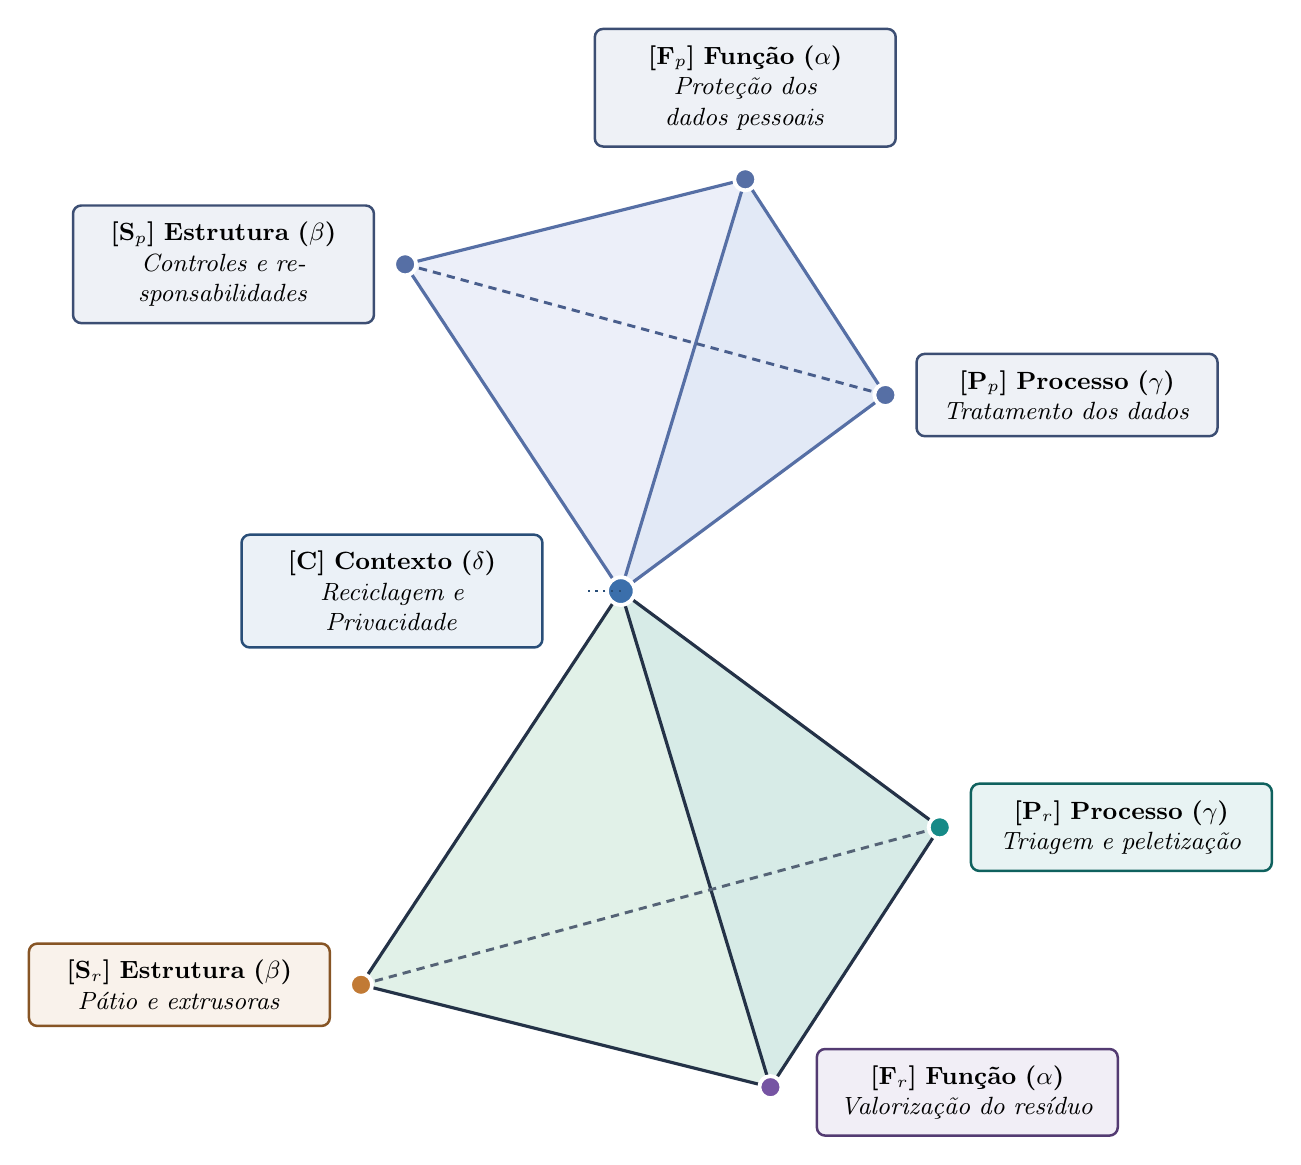
\begin{tikzpicture}[font=\sffamily]

  % ==========================================================
  % TETRAEDRO INFERIOR — RECICLAGEM
  % Coordenadas preservadas do desenho original.
  % ==========================================================
  \coordinate (C) at (0.00,4.65);
  \coordinate (S) at (-3.30,-0.35);
  \coordinate (F) at (1.90,-1.65);
  \coordinate (P) at (4.05,1.65);

  % ==========================================================
  % TETRAEDRO SUPERIOR — PRIVACIDADE
  % Silhueta do original espelhada verticalmente a partir de C
  % e reduzida para 83% de seu tamanho.
  % C não é duplicado.
  % ==========================================================
  \coordinate (Sp) at (-2.74,8.80);
  \coordinate (Fp) at (1.58,9.88);
  \coordinate (Pp) at (3.36,7.14);

  % Faces do tetraedro inferior.
  \fill[faceside, opacity=0.75]
    (C) -- (F) -- (P) -- cycle;
  \fill[facefront, opacity=0.88]
    (C) -- (S) -- (F) -- cycle;

  % Faces do tetraedro superior.
  \fill[privacyside, opacity=0.75]
    (C) -- (Fp) -- (Pp) -- cycle;
  \fill[privacyfront, opacity=0.88]
    (C) -- (Sp) -- (Fp) -- cycle;

  % Arestas visíveis da Reciclagem — mesmas do original.
  \draw[edge] (C) -- (S) -- (F) -- (P) -- cycle;
  \draw[edge] (C) -- (F);

  % Arestas visíveis da Privacidade — mesma composição visual.
  \draw[edge, draw=privacy]
    (C) -- (Sp) -- (Fp) -- (Pp) -- cycle;
  \draw[edge, draw=privacy] (C) -- (Fp);

  % Arestas posteriores tracejadas.
  \draw[hidden edge] (S) -- (P);
  \draw[hidden edge, draw=privacy!85!black] (Sp) -- (Pp);

  % Vértices da Reciclagem.
  \node[vertex, fill=str] at (S) {};
  \node[vertex, fill=fun] at (F) {};
  \node[vertex, fill=pro] at (P) {};

  % Vértices da Privacidade.
  \node[vertex, fill=privacy] at (Sp) {};
  \node[vertex, fill=privacy] at (Fp) {};
  \node[vertex, fill=privacy] at (Pp) {};

  % Único vértice de Contexto, compartilhado.
  \node[vertex, fill=con, minimum size=10pt] at (C) {};

  % ----------------------------------------------------------
  % Cartões do tetraedro superior.
  % ----------------------------------------------------------
  \node[label box=privacy, anchor=east]
    at ($(Sp)+(-0.38,0)$)
    {\textbf{[S$_p$] Estrutura ($\beta$)}\\
     \textit{Controles e responsabilidades}};

  \node[label box=privacy, anchor=south]
    at ($(Fp)+(0,0.40)$)
    {\textbf{[F$_p$] Função ($\alpha$)}\\
     \textit{Proteção dos dados pessoais}};

  \node[label box=privacy, anchor=west]
    at ($(Pp)+(0.38,0)$)
    {\textbf{[P$_p$] Processo ($\gamma$)}\\
     \textit{Tratamento dos dados}};

  % Contexto: um cartão entre os dois tetraedros.
  \draw[con!70!black, dotted, line width=0.8pt]
    (C) -- ($(C)+(-0.42,0)$);

  \node[label box=con, anchor=east]
    at ($(C)+(-0.98,0)$)
    {\textbf{[C] Contexto ($\delta$)}\\
     \textit{Reciclagem e Privacidade}};

  % ----------------------------------------------------------
  % Cartões do tetraedro inferior, próximos ao original.
  % ----------------------------------------------------------
  \node[label box=str, anchor=east]
    at ($(S)+(-0.38,0)$)
    {\textbf{[S$_r$] Estrutura ($\beta$)}\\
     \textit{Pátio e extrusoras}};

  \node[label box=fun, anchor=north]
    at ($(F)+(2.5,0.5)$)
    {\textbf{[F$_r$] Função ($\alpha$)}\\
     \textit{Valorização do resíduo}};

  \node[label box=pro, anchor=west]
    at ($(P)+(0.38,0)$)
    {\textbf{[P$_r$] Processo ($\gamma$)}\\
     \textit{Triagem e peletização}};

\end{tikzpicture}
\end{document}